% !TEX root = main.tex

\begin{figure}[ht]
\centering
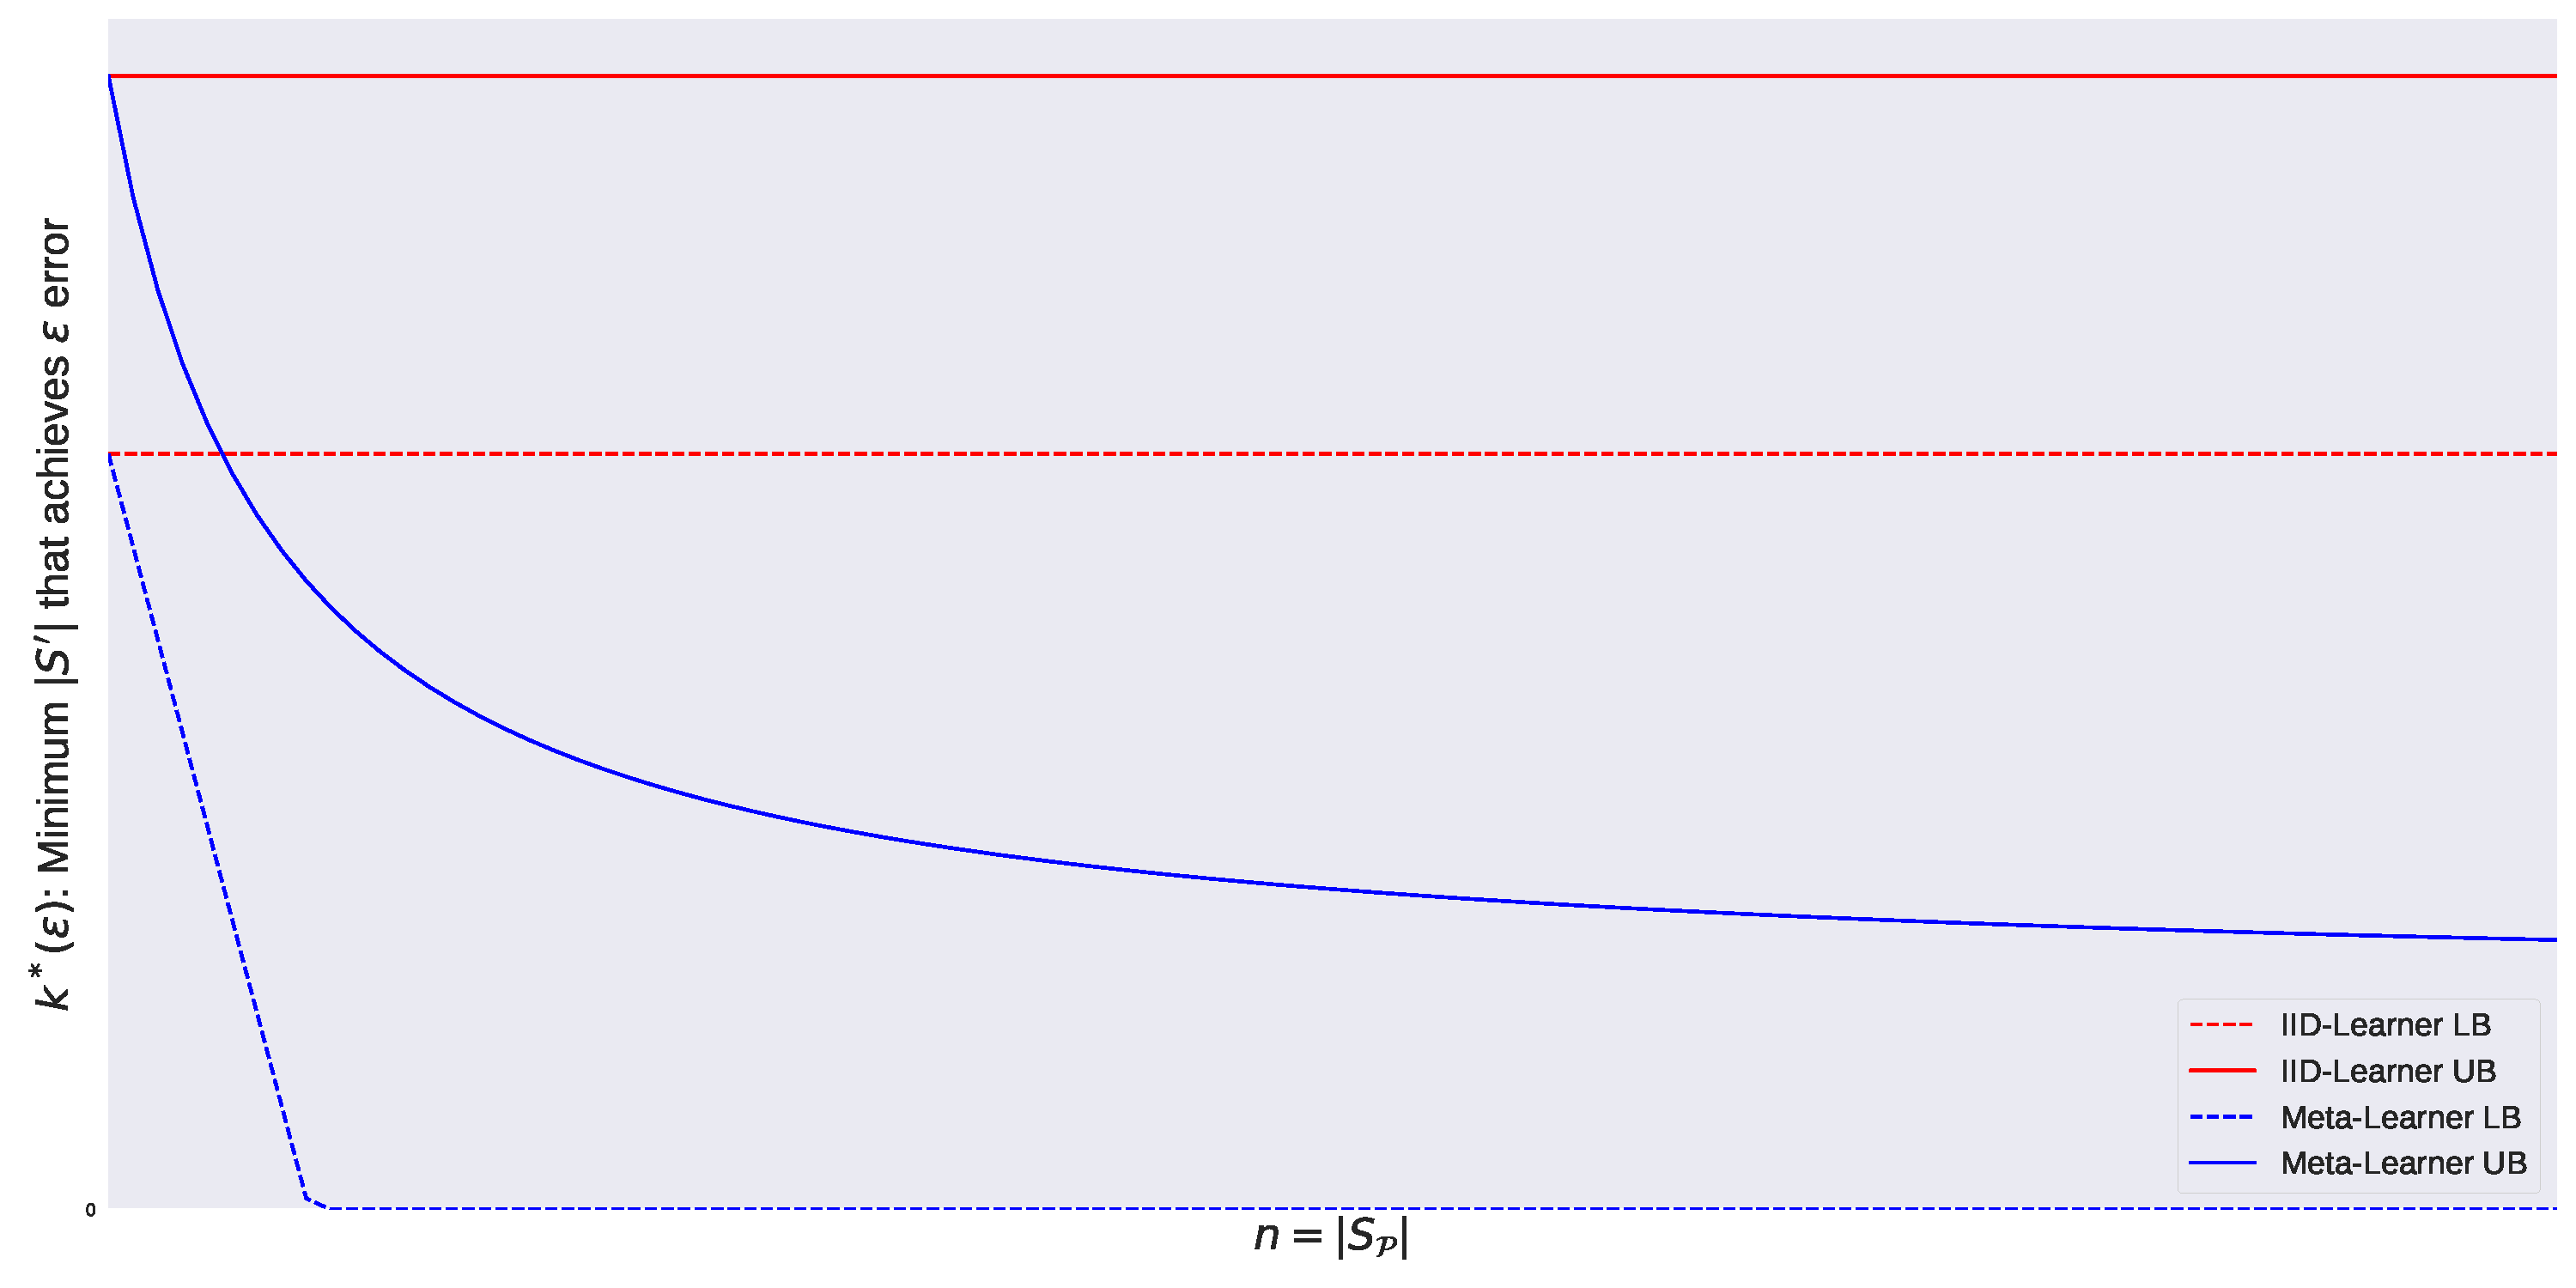
\includegraphics[width=\linewidth]{main/images/min_k_bounds_plot.pdf}\vspace{-0.5cm}
\caption{\textbf{Simulated error bounds for meta-learners} We illustrate the overall relationship between the theoretical bounds we derive in this work. On the $y$-axis, we plot the minimum number of samples needed from the novel task to achieve an $\epsilon$-error threshold. The bounds for an \iid learner that ignores the additional data, $\envS$, is shown in red while the meta-learning bounds we derive are illustrated in blue. We simulate these bounds using our derived results.
%and hand-selecting suitable constants 
Note that we chose constants to 
place the bounds for these two different learners on a similar scale, so the scale of the bounds relative to each other is uninformative.}
\label{fig:learning_bounds}
\end{figure}

\section{Summary of results}
\label{sec:summary}

\JL{Convert to bullet points in intro and remove this}

Lower bounds on the error of statistical estimation problems allow us to determine the gap between
the performance of specific learning algorithms and the theoretically best achievable error. If the
generalization upper bound and lower bound (asymptotically) match, then we know that the learning
algorithm is (asymptotically) optimal for this learning problem.

In Sections \ref{sec:minimax_setting} and \ref{sec:lbounds}, we introduce novel lower-bounds on the minimax risk of parameter estimation for a
multi-task learning problem. These lower bound characterizes the difficulty of learning in this
setting as a function of the proportion of the task-space covered by the training data, number of
training data points, and the number of data points supporting a novel task.

We then proceed in Section~\ref{sec:hierarchical_bayes} with a study of a hierarchical Bayesian model of meta linear regression. Our aims are two-fold. First, we wish to investigate the tightness of our lower bounds in this setting using an accompanying upper bound. Second, through analyzing a simple instance of the meta-learning problem we provide some intuition into the necessary conditions for successful meta-learning in general.

Figure~\ref{fig:learning_bounds} illustrates our high-level theoretical findings. We plot the minimum number of samples needed from the novel task to achieve some error threshold. The \iid-Learner does not utilize data from $\envS$ and is therefore constant. Our lower-bounds indicate that, if the training tasks sufficiently span the environment, then with enough data from these tasks the error on any novel task can be driven to zero. However, the upper bounds we derive do not have zero error asymptotically in $|\envS|$, even when the tasks may span the entire environment. We discuss this further in Section~\ref{sec:hierarchical_bayes}.

Finally, we conclude with a qualitative empirical evaluation of the meta linear regression setting. We show that this relatively simple linear setting is able to capture key features of few-shot learning and, moreover, that these features are predicted well by our theoretical analysis.